%
%                       Documento principal main.tex
%                           Plantilla de Libro            
%                             version:  0.0.2
%      
%                               Contacto:
%                 Github:   https://github.com/medicendav
%                 Correo:   davidtorrezreyes@gmail.com   
%
%-------------------------------------------------------------------------
%
%Copyright 2020 David Torrez Reyes
%This file is part of BookTemplate.
%
%BookTemplate is free software: you can redistribute it and/or modify
%it under the terms of the GNU General Public License as published by
%the Free Software Foundation, either version 3 of the License, or
%(at your option) any later version.
%
%BookTemplate is distributed in the hope that it will be useful,
%but WITHOUT ANY WARRANTY; without even the implied warranty of
%MERCHANTABILITY or FITNESS FOR A PARTICULAR PURPOSE.  See the
%GNU General Public License for more details.
%
%You should have received a copy of the GNU General Public License
%along with BookTemplete.  If not, see <https://www.gnu.org/licenses/>.
%
%-------------------------------------------------------------------------
%
%   Organización de la plantilla:
%   
%   main.tex:
%            Documento principal de la plantilla: Se cargan todos los   
%            demás archivos, como preámbulo, estilos, capítulos, etc. 
%            Este archivo es el que se compila.
%   Carpeta:
%           Estilos:
%                   preámbulo.tex:
%                          Archivo que carga todos los paquetes a utilizar.
%           Estructura:
%                   
%           Capítulos:
%
%           Imágenes:
%
%           Bibliografía:
%
%--------------------------------------------------------------------------

% Definimos la clase de documento: En este caso book, con los parámetros opcionales
% definimos el tamaÑo de letra (10pt), el tamaÑo de papel (letterpaper) y el formato
% de impresión a dos lados.
\documentclass[10pt,letterpaper,twoside]{book}


% Incluimos el archivo preámbulo,tex que se encuentra en el directorio Estilos. De
% modo que cargamos todos los paquetes necesarios para la elaboración del documento.
%
%                       Preámbulo del documento
%
%           Contiene todos los paquetes necesarios para la
%                       compilación del documento
%
%-------------------------------------------------------------------------
%
%Copyright 2020 David Torrez Reyes
%This file is part of BookTemplate.
%
%BookTemplate is free software: you can redistribute it and/or modify
%it under the terms of the GNU General Public License as published by
%the Free Software Foundation, either version 3 of the License, or
%(at your option) any later version.
%
%BookTemplate is distributed in the hope that it will be useful,
%but WITHOUT ANY WARRANTY; without even the implied warranty of
%MERCHANTABILITY or FITNESS FOR A PARTICULAR PURPOSE.  See the
%GNU General Public License for more details.
%
%You should have received a copy of the GNU General Public License
%along with BookTemplete.  If not, see <https://www.gnu.org/licenses/>.
%-------------------------------------------------------------------------




%                  Paquetes de idiomas y codificación
%-------------------------------------------------------------------------
% El paquete inputenc modifica la codificación de entrada de LaTeX.
% Permite escribir con acentos, símbolos inusuales, etc. Como parámetro 
% opcional ingresamos la codificación deseada (latin1) ISO 8859-1.  
\usepackage[utf8]{inputenc}


% El paquete babel gestiona el idioma en el cual se desea trabajar, en
% este caso español (spanish)
\usepackage[spanish]{babel}


% El paquete fontenc gestiona la codificación de salida del documento.
% EL parámetro (T1) indica la codificación estándar de LaTeX
\usepackage[T1]{fontenc}




%                  Paquetes de gráficos, tablas
%-------------------------------------------------------------------------
% El entorno multicol, es de gran utilidad en los sitios donde se
% quieren poner dos figuras una al lado de la otra.
\usepackage{multicol}


% El entorno tabularx, sirve para hacer tablas con  párrafos sin tener que
% indicar  el ancho  de cada  columna de párrafo particular.
\usepackage{tabularx}

% Paquete necesario para la adición de figuras.
% Con el comando \graphcspath indicamos el directorio en el cual se encuentran
% las imágenes a utilizar 
\usepackage{graphicx}
\graphicspath{{Imagenes/}}




%                 Paquetes de configuración de paginas 
%-------------------------------------------------------------------------
% Paquete geometry, gestiona los margenes del documento.
\usepackage[top=3cm,bottom=3cm,left=3cm,right=3cm]{geometry}
\usepackage{lipsum}



%                 Paquetes para la gestión de colores 
%-------------------------------------------------------------------------
% EL paquete xcolor, necesario para la creación y uso de colores.
\usepackage{xcolor}




%     Paquetes para la creación de ecuaciones y simbología matemática 
%-------------------------------------------------------------------------
% Paquetes necesarios para introducir simbología matemática, ecuaciones,
% teoremas, etc.
\usepackage{amsmath}
\usepackage{amsfonts}
\usepackage{amssymb}
\usepackage{amsthm}



%----------------------------------------------------------------------------
%                              Inicio del documento
%----------------------------------------------------------------------------

% Inicio del documento
\begin{document}
%
%                           	Portada
%
%           Contiene los comandos necesarios para generar la portada
%                			  del documento
%
%-------------------------------------------------------------------------
%
%Copyright 2020 David Torrez Reyes
%This file is part of BookTemplate.
%
%BookTemplate is free software: you can redistribute it and/or modify
%it under the terms of the GNU General Public License as published by
%the Free Software Foundation, either version 3 of the License, or
%(at your option) any later version.
%
%BookTemplate is distributed in the hope that it will be useful,
%but WITHOUT ANY WARRANTY; without even the implied warranty of
%MERCHANTABILITY or FITNESS FOR A PARTICULAR PURPOSE.  See the
%GNU General Public License for more details.
%
%You should have received a copy of the GNU General Public License
%along with BookTemplete.  If not, see <https://www.gnu.org/licenses/>.
%-------------------------------------------------------------------------


%----------------------------------------------
%				Primera portada
%----------------------------------------------

% Estilo de pagina vacío, No genera encabezado
\thispagestyle{empty}

% Creamos el entorno para generar portada
\begin{titlepage}
	\centering
	% Genera una linea de la longitud del texto con grosor de 1.5 pts
	\rule{\textwidth}{1.5pt} 
		% Cambio tamaño de letra grande (\huge) y texto en negritas
		% Llamamos a la constante \titulo
		{\huge\bfseries		\titulo 	\par}
	% Genera una linea de la longitud del texto con grosor de 1.5 pts
	\rule{\textwidth}{1.5pt} \par
	% Dejamos un espacio de 3cm
	\vspace{3cm}
		% Llamamos a la constante \autor y cambiamos el tamaño de letra a (Large)
		{\huge	\autor \par}
	% Deja un espacio de 3cm
	\vspace{3cm}	
		%Incluimos una imagen de portada
		{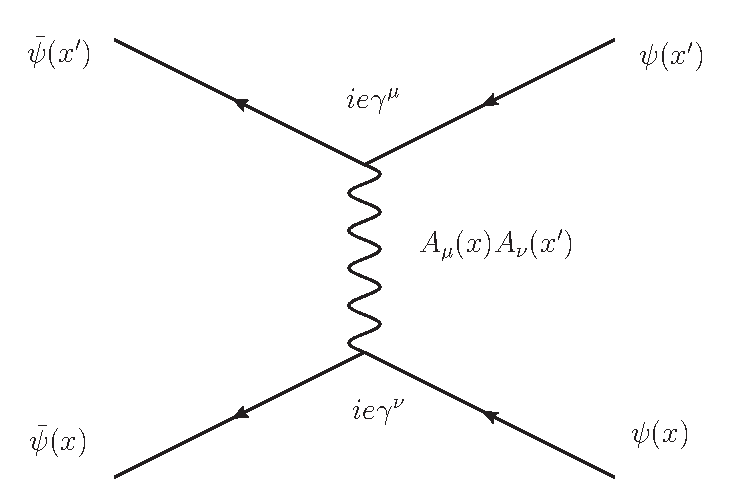
\includegraphics{diagrama_portada} \par}
		% Dejamos un espacio de 2.5cm
	\vspace{2.5cm}
		% Generamos la fecha
		{\huge	\today \par}
		% Genera una linea de la longitud del texto con grosor de 1.5 pts
	\rule{\textwidth}{1.5pt}
\end{titlepage}

%----------------------------------------------
%				Segunda portada
%----------------------------------------------

% Estilo de pagina vacío, No genera encabezado
\thispagestyle{empty}
% Creamos el entorno para generar portada
\begin{titlepage}
	\centering
	\vspace{10cm}
	% Genera una linea de la longitud del texto con grosor de 1.5 pts
	\rule{\textwidth}{1.5pt} 
		% Cambio tamaño de letra grande (\huge) y texto en negritas
		% Llamamos a la constante \titulo
		{\huge\bfseries		\titulo 	\par}
	% Genera una linea de la longitud del texto con grosor de 1.5 pts
	\rule{\textwidth}{1.5pt}
	% Termina el párrafo del titulo
	\par
	% Deja un espacio de 5cm
	\vspace{5cm}	
		{\huge Notas de Teoría Cuántica de Campos \par}
	% Deja un espacio de 5cm
	\vspace{4cm}
	% Llamamos a la constante \autor y cambiamos el tamaño de letra a (Large)
		{\huge	\autor \par}
	% Dejamos un espacio de 3cm
	\vspace{4cm}
		% Generamos la fecha
		{\Large	\today \par}
	\vspace{3cm}
		% Copyright
		{\Large \copyright{} Copyright  2020  \autor}

	\end{titlepage}

    
\end{document}